\documentclass[12pt,letterpaper]{article}

\usepackage[utf8]{inputenc}
\usepackage[T1]{fontenc}
\usepackage[english]{babel}
\usepackage{amsmath, amssymb, amsthm}
\usepackage{float, enumitem, xcolor, geometry}
\usepackage{graphicx, fancyhdr, fancyvrb}
\usepackage{array, makecell}
\usepackage{forest}
\usepackage[normalem]{ulem}
\usepackage[colorlinks=true, linkcolor=linkblue, urlcolor=linkblue, citecolor=linkblue]{hyperref}
\usepackage{makecell}
\usepackage{tikz}
\usetikzlibrary{automata, positioning, arrows.meta}

\definecolor{linkblue}{HTML}{1A167A}

\geometry{margin=2cm, top=2cm, bottom=2cm}

\newcommand{\pred}{$\rightarrow$}
\newcommand{\asig}{$\leftarrow$}

\newcommand{\nt}[1]{\textit{#1}}
\newcommand{\tk}[1]{\texttt{#1}}
\newcommand{\tx}[1]{\text{#1}}
\newcommand{\First}[1]{\mathrm{FIRST}(#1)}
\newcommand{\Follow}[1]{\mathrm{FOLLOW}(#1)}
\renewcommand{\ll}{\mathrm{LL(1)}}
\newcommand{\lr}{\mathrm{LR(1)}}
\newcommand{\lrc}{\mathrm{LR(0)}}
\newcommand{\slr}{\mathrm{SLR(1)}}
\newcommand{\lalr}{\mathrm{LALR(1)}}
\newcommand{\eps}{\varepsilon}

% ========================================
% COLORES
% ========================================
\definecolor{green}{HTML}{07E314}
\definecolor{red}{HTML}{ED4728}

% ========================================
% COMANDOS PARA MARCADORES
% ========================================
\newcommand{\greencheck}{\textcolor{green}{$\checkmark$}}
\newcommand{\redcross}{\textcolor{red}{$\times$}}
\newcommand{\conf}[1]{\textcolor{red}{#1}}
% ========================================
% CONSTANTES DEL ENCABEZADO
% ========================================
\newcommand{\encabezadoIzq}{Compiladores 2027-1}
\newcommand{\encabezadoCen}{Tarea 5}
\newcommand{\encabezadoDer}{\textit{A.S. Ascendente y Descendente}}

% ========================================
% CONFIGURACION DEL ENCABEZADO
% ========================================
\pagestyle{fancy}
\fancyhf{}

\fancyhead[L]{\encabezadoIzq}
\fancyhead[C]{\encabezadoCen}
\fancyhead[R]{\encabezadoDer}

\fancyfoot[C]{\thepage}

\renewcommand{\headrulewidth}{0.1pt}
\renewcommand{\footrulewidth}{0pt}

% ========================================
% CONFIGURACION DE TABLAS
% ========================================
\newcolumntype{C}[1]{>{\centering\arraybackslash}m{#1}}
\newcolumntype{L}[1]{>{\raggedright\arraybackslash}m{#1}}
\newcolumntype{R}[1]{>{\raggedleft\arraybackslash}m{#1}}

\begin{document}

\thispagestyle{empty}
\begin{titlepage}
  \thispagestyle{empty}
  %--------------- COMANDO LINEA----------------->
  \newcommand{\linea}{\rule{\linewidth}{0.5mm}}                 
  \center
  %<<<<<<<<<<<<<<<<<<<<<<<<<<<<<<<<<<<<<<<<<<<

  %Add logos
  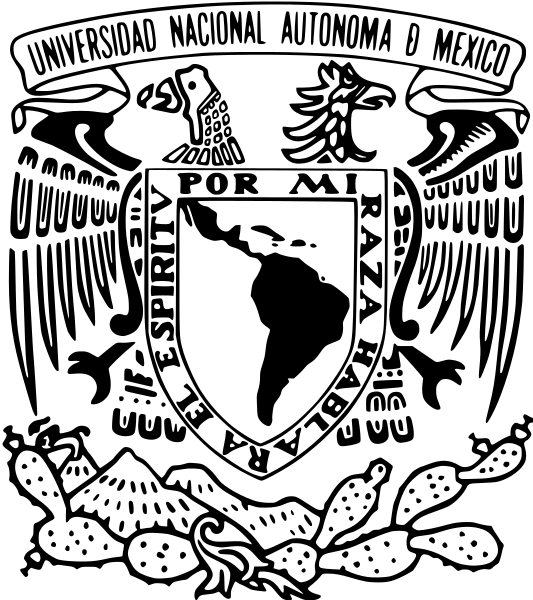
\includegraphics[width=0.24\textwidth]{../unam_logo.png} \hspace{1.5cm}
  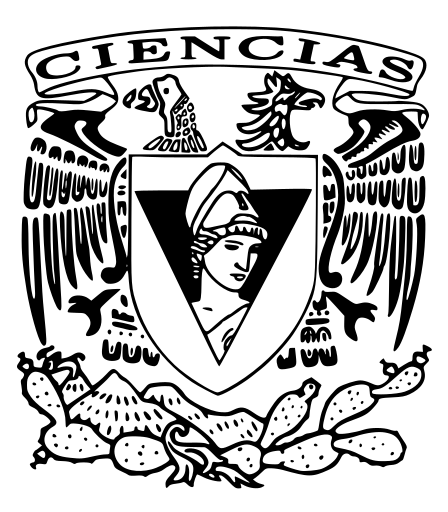
\includegraphics[width=0.25\textwidth]{../fc_logo.png} \\[1cm]
  \textbf{\Large UNIVERSIDAD NACIONAL AUTÓNOMA}\\[3mm]
  \textbf{\Large DE MÉXICO} \\[6mm]
  \textit{\Large Facultad de Ciencias}

  \vfill

  %---------------TÍTULO----------------->
  \linea
  \vfill \vspace{1cm}
  \textbf{\Large Compiladores}\\[1.1cm]
  \textbf{\Large Análisis sintáctico Descendente y Ascendente}\\[0.9cm]
  \linea \\
  \vfill
  \vspace{0.7cm}
  %Title of the Research
  \textbf{\Large  Tarea 5}\\[6mm]
  %<<<<<<<<<<<<<<<<<<<<<<<<<<<<<<<<<<<<<<<<<<<

  %Team
  \vfill
  \textit{\small Presenta:}\\
  \textbf{\large  \textbf{Ramírez Juárez María Fernanda} - 321204747}\\[3mm]
  \textbf{\large  \textbf{Rojo Peña Manuel Ianluck} - 118005762}\\[3mm]

  %Profesor y Grupo
  \textit{\small Profesor:}\\
  \textbf{Pablo Martínez Yessica Janeth}\\[3mm]
  \textit{\small Ayudante:}\\
  \textbf{Rojas Fuentes Andrea}\\[3mm]
  \small Grupo: 7010, 2027-1\\[3mm]
  \vfill

  %Fecha or Date
  \textit{\small Fecha de entrega:}\\
         {\large 22 de octubre, 2026}
         
\end{titlepage}


%%%%%%%%%%%%%%%%%%%%%%%%%%%%%%%%%%%%%%%%%%
\newpage
%%%%%%%%%%%%%%%%%%%%%%%%%%%%%%%%%%%%%%%%%%

\begin{enumerate}[label=\arabic*.]

\item Muestre que la siguiente gramática es $\ll$ pero no $\slr$
  \[
  \begin{aligned}
    \nt{S} &\to \tx{A}\ \tk{a}\ \tx{A}\ \tk{b}\ \mid \tx{B}\ \tk{b}\ \tx{B}\ \tk{a} \\
    \nt{A} &\to \eps \\
    \nt{B} &\to \eps
  \end{aligned}
  \]

  %%%%%%%%%%%%%%%%%%%%%%%%%%
  \bigskip
  %%%%%%%%%%%%%%%%%%%%%%%%%%
  
  \boxed{\textbf{\large P.D.}}\ \textbf{\large La gramática es $\ll$}\\

  \textbf{Paso 1. Anulables}\\
  \nt{A} y \nt{B} son anulables porque tienen la producción $\eps$, pero \nt{S} no es anulable, pues
  cualquiera de sus dos alternativas contiene terminales (\tk{a}, \tk{b}) que siempre deben generarse.\\

  \textbf{Paso 2. \textsc{First}}\\
  Partimos de lo que no depende de nadie:
  \[
  \First{\nt{A}} = \{\eps\} \qquad \First{\nt{B}} = \{\eps\}
  \]

  Para cada alternativa de \nt{S} recorremos el lado derecho de izquierda a derecha, avanzando mientras el
  símbolo sea anulable:
  \[
  \begin{aligned}
    \First{\nt{A}\,\tk{a}\,\nt{A}\,\tk{b}}
    &= \big(\First{\nt{A}}\setminus\{\eps\}\big) \cup \First{\tk{a}}
    = \varnothing \cup \{\tk{a}\} = \{\tk{a}\} \\
    \First{\nt{B}\,\tk{b}\,\nt{B}\,\tk{a}}
    &= \big(\First{\nt{B}}\setminus\{\eps\}\big) \cup \First{\tk{b}}
    = \varnothing \cup \{\tk{b}\} = \{\tk{b}\}
  \end{aligned}
  \]
  El recorrido se detiene en el terminal porque no es anulable, entonces $\First{\nt{S}}$ es la
  \textbf{unión} de ambas alternativas:
  \[
  \First{\nt{S}} = \{\tk{a}\} \cup \{\tk{b}\} = \{\tk{a},\ \tk{b}\}
  \]

  \textbf{Paso 3. \textsc{Follow}}
  \begin{itemize}
  \item $\Follow{\tx{S}}$: como es el símbolo inicial aporta \tk{\$}, no aparece en ningún lado derecho.
    \[
    \Follow{\nt{S}} = \{\tk{\$}\}
    \]

  \item $\Follow{\tx{A}}$: aparece dos veces en $\nt{S}\to\nt{A}\,\tk{a}\,\nt{A}\,\tk{b}$.\\
    A la primera \nt{A} le sigue $\tk{a}\,\nt{A}\,\tk{b}$, cuyo $\mathrm{FIRST}$ es $\{\tk{a}\}$
    (como ya mostramos).\\
    A la segunda \nt{A} le sigue \tk{b}.\\
    \nt{A} nunca queda al final de una producción, así que no hereda $\Follow{\nt{S}}$.
    \[
    \Follow{\nt{A}} = \{\tk{a},\ \tk{b}\}
    \]

  \item $\Follow{\tx{B}}$: aparece dos veces en $\nt{S}\to\nt{B}\,\tk{b}\,\nt{B}\,\tk{a}$.\\
    A la primera \nt{B} le sigue $\tk{b}\,\nt{B}\,\tk{a}$, que aporta \tk{b}.\\
    A la segunda \nt{B} le sigue \tk{a}.\\
    Tampoco queda al final de ninguna producción.
    \[
    \Follow{\nt{B}} = \{\tk{a},\ \tk{b}\}
    \]
  \end{itemize}

  Al repetir las reglas ningún conjunto vuelve a cambiar, por lo que ya es el punto fijo.\\

  Por lo tanto, los conjuntos \textsc{First} y \textsc{Follow} de la gramática son:
  \[
  \begin{aligned}
    \First{\nt{S}} &= \{\tk{a},\ \tk{b}\} & \Follow{\nt{S}} &= \{\tk{\$}\} \\
    \First{\nt{A}} &= \{\eps\}            & \Follow{\nt{A}} &= \{\tk{a},\ \tk{b}\} \\
    \First{\nt{B}} &= \{\eps\}            & \Follow{\nt{B}} &= \{\tk{a},\ \tk{b}\}
  \end{aligned}
  \]

  \textbf{Paso 4. Producciones enumeradas y su selección}
  \[
  \begin{array}{c l l l}
    \# & \text{Producción} & \text{Colocado en} & \text{Motivo} \\ \hline
    1 & \nt{S}\to\nt{A}\,\tk{a}\,\nt{A}\,\tk{b} & \tk{a} & \First{\nt{A}\,\tk{a}\,\nt{A}\,\tk{b}} \\
    2 & \nt{S}\to\nt{B}\,\tk{b}\,\nt{B}\,\tk{a} & \tk{b} & \First{\nt{B}\,\tk{b}\,\nt{B}\,\tk{a}} \\
    3 & \nt{A}\to\eps & \tk{a},\tk{b} & \Follow{\nt{A}} \\
    4 & \nt{B}\to\eps & \tk{a},\tk{b} & \Follow{\nt{B}}
  \end{array}
  \]

  \textbf{Paso 5. Tabla $\ll$}
  \[
  \begin{array}{c|c|c|c}
    & \tk{a} & \tk{b} & \tk{\$} \\ \hline
    \nt{S} & 1 & 2 &   \\ \hline
    \nt{A} & 3 & 3 &   \\ \hline
    \nt{B} & 4 & 4 &   \\
  \end{array}
  \]

  Ninguna celda tiene más de una producción, por ejemplo para \nt{S}, las dos alternativas
  tienen $\First$ disjuntos:
  \[
  \First{\nt{A}\,\tk{a}\,\nt{A}\,\tk{b}} \cap \First{\nt{B}\,\tk{b}\,\nt{B}\,\tk{a}}
  = \{\tk{a}\} \cap \{\tk{b}\} = \varnothing
  \]
  Y \nt{A} y \nt{B} tienen una sola producción cada una, así que no pueden chocar consigo mismas.\\

  Por lo tanto \textbf{La gramática es $\ll$.}

  %%%%%%%%%%%%%%%%%%%%%%%%
  \bigskip
  %%%%%%%%%%%%%%%%%%%%%%%%
  
  \boxed{\textbf{\large P.D.}}\ \textbf{\large La gramática no es $\slr$}\\

  \textbf{Paso 1. Gramática aumentada}\\
  Agregamos un nuevo símbolo inicial $\nt{S'}$ y se enumeramos las producciones:
  \[
  \begin{aligned}
    (0)\ & \nt{S'} &\to \nt{S} \\
    (1)\ & \nt{S}  &\to \nt{A}\,\tk{a}\,\nt{A}\,\tk{b} \\
    (2)\ & \nt{S}  &\to \nt{B}\,\tk{b}\,\nt{B}\,\tk{a} \\
    (3)\ & \nt{A}  &\to \eps \\
    (4)\ & \nt{B}  &\to \eps
  \end{aligned}
  \]

  \textbf{Paso 2. Cerrradura y AFD de ítems $\mathrm{LR(0)}$ (\texttt{goto})}\\
  Una producción $\nt{A}\to\eps$ genera directamente el ítem completo $\nt{A}\to\bullet$, el punto ya está al
  final, por lo que en el estado inicial hay dos reducciones posibles.\\
  \[
  \textbf{closure}\big(\{\nt{S'}\to\bullet\,\nt{S}\}\big)
  \]
  el punto está antes de \nt{S}, se agregan sus dos producciones; en ellas el punto queda antes de \nt{A} y de
  \nt{B}, se agregan $\nt{A}\to\bullet$ y $\nt{B}\to\bullet$.

  \medskip

  \textbf{Estado:}
  \[
  \begin{aligned}
    I_0 = \{\, & \nt{S'} \to \bullet\,\nt{S},\\
               & \nt{S}  \to \bullet\,\nt{A}\,\tk{a}\,\nt{A}\,\tk{b},\\
               & \nt{S}  \to \bullet\,\nt{B}\,\tk{b}\,\nt{B}\,\tk{a},\\
               & \nt{A}  \to \bullet,\\
               & \nt{B}  \to \bullet\,\}
  \end{aligned}
  \]

  \textbf{Transiciones:}
  \[
  \begin{aligned}
    X=\nt{S}:\ \texttt{goto}(I_0,\nt{S}) &= \{\,\nt{S'}\to\nt{S}\,\bullet\,\} = \boxed{I_1}\\[3pt]
    X=\nt{A}:\ \texttt{goto}(I_0,\nt{A}) &= \{\,\nt{S}\to\nt{A}\,\bullet\,\tk{a}\,\nt{A}\,\tk{b}\,\}
    = \boxed{I_2}\\[3pt]
    X=\nt{B}:\ \texttt{goto}(I_0,\nt{B}) &= \{\,\nt{S}\to\nt{B}\,\bullet\,\tk{b}\,\nt{B}\,\tk{a}\,\}
    = \boxed{I_3}
  \end{aligned}
  \]

  \medskip

  \textbf{Estado:}\quad $I_1 = \{\,\nt{S'}\to\nt{S}\,\bullet\,\}$\\
  Es el estado de aceptación, no tiene transiciones.

  \medskip

  \textbf{Estado:}\quad $I_2 = \{\,\nt{S}\to\nt{A}\,\bullet\,\tk{a}\,\nt{A}\,\tk{b}\,\}$

  \textbf{Transiciones:}
  \[
  \begin{aligned}
    X=\tk{a}:\ \texttt{goto}(I_2,\tk{a}) = \{\, & \nt{S}\to\nt{A}\,\tk{a}\,\bullet\,\nt{A}\,\tk{b},\\
                                              & \nt{A}\to\bullet\,\} = \boxed{I_4}
  \end{aligned}
  \]
  El ítem $\nt{A}\to\bullet$ viene de la cerradura, el punto quedó antes de \nt{A}.

  \medskip

  \textbf{Estado:}\quad $I_3 = \{\,\nt{S}\to\nt{B}\,\bullet\,\tk{b}\,\nt{B}\,\tk{a}\,\}$

  \textbf{Transiciones:}
  \[
  \begin{aligned}
    X=\tk{b}:\ \texttt{goto}(I_3,\tk{b}) = \{\, & \nt{S}\to\nt{B}\,\tk{b}\,\bullet\,\nt{B}\,\tk{a},\\
                                              & \nt{B}\to\bullet\,\} = \boxed{I_7}
  \end{aligned}
  \]

  \medskip

  \textbf{Estado:}
  \[
  \begin{aligned}
    I_4 = \{\, & \nt{S}\to\nt{A}\,\tk{a}\,\bullet\,\nt{A}\,\tk{b},\\
               & \nt{A}\to\bullet\,\}
  \end{aligned}
  \]

  \textbf{Transiciones:} el ítem $\nt{A}\to\bullet$ ya está completo, no avanza.
  \[
  X=\nt{A}:\ \texttt{goto}(I_4,\nt{A}) = \{\,\nt{S}\to\nt{A}\,\tk{a}\,\nt{A}\,\bullet\,\tk{b}\,\} = \boxed{I_5}
  \]

  \medskip

  \textbf{Estado:}\quad $I_5 = \{\,\nt{S}\to\nt{A}\,\tk{a}\,\nt{A}\,\bullet\,\tk{b}\,\}$

  \textbf{Transiciones:}
  \[
  X=\tk{b}:\ \texttt{goto}(I_5,\tk{b}) = \{\,\nt{S}\to\nt{A}\,\tk{a}\,\nt{A}\,\tk{b}\,\bullet\,\} = \boxed{I_6}
  \]

  \medskip

  \textbf{Estado:}\quad $I_6 = \{\,\nt{S}\to\nt{A}\,\tk{a}\,\nt{A}\,\tk{b}\,\bullet\,\}$\\
  Ítem completo, no tiene transiciones.

  \medskip

  \textbf{Estado:}
  \[
  \begin{aligned}
    I_7 = \{\, & \nt{S}\to\nt{B}\,\tk{b}\,\bullet\,\nt{B}\,\tk{a},\\
               & \nt{B}\to\bullet\,\}
  \end{aligned}
  \]

  \textbf{Transiciones:}
  \[
  X=\nt{B}:\ \texttt{goto}(I_7,\nt{B}) = \{\,\nt{S}\to\nt{B}\,\tk{b}\,\nt{B}\,\bullet\,\tk{a}\,\} = \boxed{I_8}
  \]

  \medskip

  \textbf{Estado:}\quad $I_8 = \{\,\nt{S}\to\nt{B}\,\tk{b}\,\nt{B}\,\bullet\,\tk{a}\,\}$

  \textbf{Transiciones:}
  \[
  X=\tk{a}:\ \texttt{goto}(I_8,\tk{a}) = \{\,\nt{S}\to\nt{B}\,\tk{b}\,\nt{B}\,\tk{a}\,\bullet\,\} = \boxed{I_9}
  \]

  \medskip

  \textbf{Estado:}\quad $I_9 = \{\,\nt{S}\to\nt{B}\,\tk{b}\,\nt{B}\,\tk{a}\,\bullet\,\}$\\
  Ítem completo, no tiene transiciones.\\

  \textbf{Paso 3. Tabla $\slr$}\\
  Reglas para llenarla:

  \begin{itemize}
  \item \textbf{Desplazar} ($d_N$): solo viene de un \texttt{goto} con terminal.
    Si $\texttt{goto}(I_k,x)=I_N$, entonces $\mathrm{ACCION}[k,x]=d_N$.
    
  \item \textbf{GOTO}: si $\texttt{goto}(I_k,\nt{X})=I_N$ con \nt{X} no terminal,
    entonces $\mathrm{GOTO}[k,\nt{X}]=N$.
    
  \item \textbf{Reducir} ($r_j$): solo para ítems con el punto al final, $\nt{X}\to\alpha\,\bullet$,
    donde $j$ es el número de la producción. En $\slr$ se coloca únicamente en las columnas de $\Follow{\nt{X}}$.

  \item \textbf{Aceptar}: el estado que contiene $\nt{S'}\to\nt{S}\,\bullet$ lleva \textit{aceptar} en la
    columna \tk{\$}.
  \end{itemize}
  
  Del \textbf{Paso 3} donde mostramos que es $\ll$:\\
  $\Follow{\nt{S}}=\{\tk{\$}\}$ y $\Follow{\nt{A}}=\Follow{\nt{B}}=\{\tk{a},\tk{b}\}$.
  \[
  \begin{array}{c|c|c|c||c|c|c}
    & \multicolumn{3}{c||}{\text{Acción}} & \multicolumn{3}{c}{\text{GOTO}} \\ \hline
    \text{Estado} & \tk{a} & \tk{b} & \tk{\$} & \nt{S} & \nt{A} & \nt{B} \\ \hline
    0 & \conf{r3/r4} & \conf{r3/r4} &   & 1 & 2 & 3 \\ \hline
    1 &    &    & \text{aceptar} &   &   &   \\ \hline
    2 & d4 &    &    &   &   &   \\ \hline
    3 &    & d7 &    &   &   &   \\ \hline
    4 & r3 & r3 &    &   & 5 &   \\ \hline
    5 &    & d6 &    &   &   &   \\ \hline
    6 &    &    & r1 &   &   &   \\ \hline
    7 & r4 & r4 &    &   &   & 8 \\ \hline
    8 & d9 &    &    &   &   &   \\ \hline
    9 &    &    & r2 &   &   &   \\
  \end{array}
  \]

  \textbf{Paso 4. Conflicto}\\
  En $I_0$ hay dos ítems completos: $\nt{A}\to\bullet$ y $\nt{B}\to\bullet$.\\
  En $\slr$, cada reducción se coloca en su $\mathrm{FOLLOW}$:
  \[
  \Follow{\nt{A}} \cap \Follow{\nt{B}} = \{\tk{a},\tk{b}\} \cap \{\tk{a},\tk{b}\} = \{\tk{a},\ \tk{b}\} \neq \varnothing
  \]
  Por lo tanto $\mathrm{ACCION}[0,\tk{a}] = \{r3,\ r4\}$ y $\mathrm{ACCION}[0,\tk{b}] = \{r3,\ r4\}$, hay un
  \textbf{conflicto reducción/reducción} en $I_0$. Los demás estados no tienen conflictos.\\

  \textbf{Observación.} $\ll$ sí distingue ambas producciones porque decide con el $\First$ de todo el lado
  derecho, y ahí \tk{a} y \tk{b} son distintos. $\slr$, en cambio, debe elegir qué $\eps$ reducir
  usando solo $\mathrm{FOLLOW}$, que mezcla todos los contextos donde aparece \nt{A} (o \nt{B}) y los vuelve
  indistinguibles.\\

  De este modo \textbf{La gramática no es $\slr$.}\\

  \text{\large Por lo tanto la gramática es $\ll$ pero no $\slr$.}

  
%%%%%%%%%%%%%%%%%%%%%%%%%%%%%%%%%%%%%%%%%%
\newpage
%%%%%%%%%%%%%%%%%%%%%%%%%%%%%%%%%%%%%%%%%%


\item Muestre que la siguiente gramática es $\slr$ pero no $\ll$
  \[
  \begin{aligned}
    \nt{S} &\to \tx{S}\ \tx{A}\ \mid \tx{A} \\
    \nt{A} &\to \tk{a} 
  \end{aligned}
  \]
 
  %%%%%%%%%%%%%%%%%%%%%%%%%%
  \bigskip
  %%%%%%%%%%%%%%%%%%%%%%%%%%

  \boxed{\textbf{\large P.D.}}\ \textbf{\large La gramática no es $\ll$}\\

  \textbf{Paso 1. Anulables}\\
  Ningún no terminal tiene la producción $\eps$ ni deriva en ella, así que no hay anulables.\\

  \textbf{Paso 2. \textsc{First}}\\
  \[
  \First{\nt{A}} = \{\tk{a}\}
  \]
  Para \nt{S}, la alternativa $\nt{S}\to\nt{S}\,\nt{A}$ empieza con la \nt{S} misma (recursión por la izquierda),
  así que solo aporta $\First{\nt{S}}$, que no agrega nada nuevo.\\
  La alternativa $\nt{S}\to\nt{A}$ aporta $\First{\nt{A}}$:
  \[
  \First{\nt{S}} = \First{\nt{S}} \cup \First{\nt{A}} = \{\tk{a}\}
  \]

  \textbf{Paso 3. \textsc{Follow}}
  \begin{itemize}
  \item $\Follow{\tx{S}}$: es el símbolo inicial, así que aporta \tk{\$}.\\
    En $\nt{S}\to\nt{S}\,\nt{A}$ le sigue \nt{A} que no es anulable, así que se agrega
    $\First{\nt{A}} = \{\tk{a}\}$.
    \[
    \Follow{\nt{S}} = \{\tk{\$},\ \tk{a}\}
    \]

  \item $\Follow{\tx{A}}$: aparece al final de $\nt{S}\to\nt{S}\,\nt{A}$ y de $\nt{S}\to\nt{A}$, así que hereda
    $\Follow{\nt{S}}$ en ambas.
    \[
    \Follow{\nt{A}} = \{\tk{\$},\ \tk{a}\}
    \]
  \end{itemize}

  Por lo tanto, los conjuntos \textsc{First} y \textsc{Follow} de la gramática son:
  \[
  \begin{aligned}
    \First{\nt{S}} &= \{\tk{a}\} & \Follow{\nt{S}} &= \{\tk{\$},\ \tk{a}\} \\
    \First{\nt{A}} &= \{\tk{a}\} & \Follow{\nt{A}} &= \{\tk{\$},\ \tk{a}\}
  \end{aligned}
  \]

  \textbf{Paso 4. Producciones enumeradas y su selección}
  \[
  \begin{array}{c l l l}
    \# & \text{Producción} & \text{Colocado en} & \text{Motivo} \\ \hline
    1 & \nt{S}\to\nt{S}\,\nt{A} & \tk{a} & \First{\nt{S}\,\nt{A}} \\
    2 & \nt{S}\to\nt{A} & \tk{a} & \First{\nt{A}} \\
    3 & \nt{A}\to\tk{a} & \tk{a} & \First{\tk{a}}
  \end{array}
  \]

  \textbf{Paso 5. Tabla $\ll$}
  \[
  \begin{array}{c|c|c}
    & \tk{a} & \tk{\$} \\ \hline
    \nt{S} & \conf{1,\ 2} & \\ \hline
    \nt{A} & 3 & \\
  \end{array}
  \]

  La celda $M[\nt{S},\tk{a}]$ tiene dos producciones, porque los $\First$ de las dos alternativas de \nt{S}
  no son disjuntos:
  \[
  \First{\nt{S}\,\nt{A}} \cap \First{\nt{A}} = \{\tk{a}\} \cap \{\tk{a}\} = \{\tk{a}\} \neq \varnothing
  \]
  La causa es la recursión por la izquierda en \nt{S}, pues ningún analizador descendente con un símbolo de
  anticipación puede decidir cuál alternativa usar viendo solo \tk{a}.\\

  Por lo tanto \textbf{La gramática no es $\ll$.}

  %%%%%%%%%%%%%%%%%%%%%%
  \bigskip
  %%%%%%%%%%%%%%%%%%%%%%

  \boxed{\textbf{\large P.D.}}\ \textbf{\large La gramática es $\slr$}\\

  \textbf{Paso 1. Gramática aumentada}
  \[
  \begin{aligned}
    (0)\ & \nt{S'} \to \nt{S} \\
    (1)\ & \nt{S} \to \nt{S}\,\nt{A} \\
    (2)\ & \nt{S} \to \nt{A} \\
    (3)\ & \nt{A} \to \tk{a}
  \end{aligned}
  \]
  Además, $\Follow{\nt{S'}} = \{\tk{\$}\}$.\\

  \textbf{Paso 2. Cerradura y AFD de ítems $\mathrm{LR(0)}$ (\texttt{goto})}\\[4pt]

  \[
  \textbf{closure}\big(\{\nt{S'}\to\bullet\,\nt{S}\}\big)
  \]
  El punto está antes de \nt{S}, se agregan $\nt{S}\to\bullet\,\nt{S}\,\nt{A}$ y $\nt{S}\to\bullet\,\nt{A}$;
  en la segunda el punto queda antes de \nt{A}, se agrega $\nt{A}\to\bullet\,\tk{a}$.

  \medskip

  \textbf{Estado:}
  \[
  \begin{aligned}
    I_0 = \{\, & \nt{S'}\to\bullet\,\nt{S},\\
               & \nt{S}\to\bullet\,\nt{S}\,\nt{A},\\
               & \nt{S}\to\bullet\,\nt{A},\\
               & \nt{A}\to\bullet\,\tk{a}\,\}
  \end{aligned}
  \]

  \textbf{Transiciones:}
  \[
  \begin{aligned}
    X=\nt{S}:\ \texttt{goto}(I_0,\nt{S}) = \{\, & \nt{S'}\to\nt{S}\,\bullet,\\
                                              & \nt{S}\to\nt{S}\,\bullet\,\nt{A},\\
                                              & \nt{A}\to\bullet\,\tk{a}\,\} = \boxed{I_1}
  \end{aligned}
  \]
  Al avanzar el punto sobre \nt{S} en $\nt{S}\to\bullet\,\nt{S}\,\nt{A}$ el punto queda antes de \nt{A}, por
  eso la cerradura agrega $\nt{A}\to\bullet\,\tk{a}$.
  \[
  \begin{aligned}
    X=\nt{A}:\ \texttt{goto}(I_0,\nt{A}) &= \{\,\nt{S}\to\nt{A}\,\bullet\,\} = \boxed{I_2}\\[3pt]
    X=\tk{a}:\ \texttt{goto}(I_0,\tk{a}) &= \{\,\nt{A}\to\tk{a}\,\bullet\,\} = \boxed{I_3}
  \end{aligned}
  \]

  \medskip

  \textbf{Estado:}
  \[
  \begin{aligned}
    I_1 = \{\, & \nt{S'}\to\nt{S}\,\bullet,\\
               & \nt{S}\to\nt{S}\,\bullet\,\nt{A},\\
               & \nt{A}\to\bullet\,\tk{a}\,\}
  \end{aligned}
  \]
  Contiene $\nt{S'}\to\nt{S}\,\bullet$, así que aquí va \textit{aceptar}.

  \textbf{Transiciones:} $\nt{S'}\to\nt{S}\,\bullet$ ya está completo, no avanza.
  \[
  \begin{aligned}
    X=\nt{A}:\ \texttt{goto}(I_1,\nt{A}) &= \{\,\nt{S}\to\nt{S}\,\nt{A}\,\bullet\,\} = \boxed{I_4}\\[3pt]
    X=\tk{a}:\ \texttt{goto}(I_1,\tk{a}) &= \{\,\nt{A}\to\tk{a}\,\bullet\,\} = I_3
  \end{aligned}
  \]

  \medskip

  \textbf{Estado:}\quad $I_2 = \{\,\nt{S}\to\nt{A}\,\bullet\,\}$\\
  Ítem completo, no tiene transiciones.

  \medskip

  \textbf{Estado:}\quad $I_3 = \{\,\nt{A}\to\tk{a}\,\bullet\,\}$\\
  Ítem completo, no tiene transiciones.

  \medskip

  \textbf{Estado:}\quad $I_4 = \{\,\nt{S}\to\nt{S}\,\nt{A}\,\bullet\,\}$\\
  Ítem completo, no tiene transiciones.\\

  \textbf{Paso 3. Tabla $\slr$}\\
  Reglas para llenarla:
  \begin{itemize}
  \item \textbf{Desplazar} ($d_N$): solo viene de un \texttt{goto} con terminal. Si
    $\texttt{goto}(I_k,x)=I_N$, entonces $\mathrm{ACCION}[k,x]=d_N$.
  \item \textbf{GOTO}: si $\texttt{goto}(I_k,\nt{X})=I_N$ con \nt{X} no terminal, entonces $\mathrm{GOTO}[k,\nt{X}]=N$.
  \item \textbf{Reducir} ($r_j$): solo para ítems con el punto al final, $\nt{X}\to\alpha\,\bullet$, donde $j$ es el
    número de la producción. En $\slr$ se coloca únicamente en las columnas de $\Follow{\nt{X}}$.
  \item \textbf{Aceptar}: el estado que contiene $\nt{S'}\to\nt{S}\,\bullet$ lleva \textit{aceptar} en la columna \tk{\$}.
  \end{itemize}
  Del Paso 3 de la Parte A: $\Follow{\nt{S}}=\Follow{\nt{A}}=\{\tk{a},\tk{\$}\}$.
  \[
  \begin{array}{c|c|c||c|c}
    & \multicolumn{2}{c||}{\text{Acción}} & \multicolumn{2}{c}{\text{GOTO}} \\ \hline
    \text{Estado} & \tk{a} & \tk{\$} & \nt{S} & \nt{A} \\ \hline
    0 & d3 &    & 1 & 2 \\ \hline
    1 & d3 & \text{aceptar} &   & 4 \\ \hline
    2 & r2 & r2 &   &   \\ \hline
    3 & r3 & r3 &   &   \\ \hline
    4 & r1 & r1 &   &   \\
  \end{array}
  \]

  \textbf{Paso 4. Verificación de conflictos}\\
  Solo $I_1$ mezcla un ítem completo con un ítem de desplazamiento, $\nt{S'}\to\nt{S}\,\bullet$ se acepta en
  \tk{\$} y $\nt{A}\to\bullet\,\tk{a}$ desplaza con \tk{a}. Son columnas distintas, así que no hay conflicto.
  $I_2$, $I_3$ e $I_4$ tienen un solo ítem completo y ningún desplazamiento. Ninguna celda tiene más de una
  acción.\\

  De este modo \textbf{La gramática es $\slr$}.\\

  Por lo tanto es $\slr$ pero no $\ll$.
  
%%%%%%%%%%%%%%%%%%%%%%%%%%%%%%%%%%%%%%%%%%
\newpage
%%%%%%%%%%%%%%%%%%%%%%%%%%%%%%%%%%%%%%%%%%


\item Dadas las siguientes gramáticas:
  \begin{itemize}
  \item Gramática 1:
    \[
    \begin{aligned}
      \nt{E} &\to \tk{(}\ \tx{L}\ \tk{)}\ \mid \tk{a} \\
      \nt{L} &\to \tx{L}\ \tk{,}\ \tx{E}\ \mid \tx{E}
    \end{aligned}
    \]
    
  \item Gramática 2:
    \[
    \begin{aligned}
      \nt{A} &\to \tx{A}\ \tk{(}\ \tx{A}\ \tk{)} \mid \eps
    \end{aligned}
    \]
  \end{itemize}

  \begin{enumerate}[label=\alph*.]
    \item Construya el \textbf{AFD} de elementos $\lrc$.
    \item Construya la tabla de análisis sintáctico $\slr$.
    \item Muestre la pila de análisis sintáctico y las acciones de un analizador $\slr$ para la cadena:
      \begin{itemize}
      \item \tk{(}\ \tk{(a),}\ \tk{a,}\ \tk{(a,a)}\ \tk{)}\; para la gramática 1
        
      \item \tk{(}\ \tk{(}\ \tk{)}\ \tk{(}\ \tk{)}\ \tk{)}\; para la gramática 2
      \end{itemize}
      
    \item ¿Esta gramática es $\lrc$? Si no es así, describa el conflicto $\lrc$. Si lo es, construya la tabla de
      análisis sintáctico $\lrc$.
  \end{enumerate}
  
  %%%%%%%%%%%%%%%%%%%%%%%%%%
  \bigskip
  %%%%%%%%%%%%%%%%%%%%%%%%%%
  

  
  
%%%%%%%%%%%%%%%%%%%%%%%%%%%%%%%%%%%%%%%%%%
\newpage
%%%%%%%%%%%%%%%%%%%%%%%%%%%%%%%%%%%%%%%%%%


\item Considere las gramáticas del ejercicio anterior y para cada una de ellas:
  \begin{enumerate}[label=\alph*.]
    \item Construya el \textbf{AFD} de elementos $\lr$
    \item Construya la tabla de análisis sintáctico $\lr$
    \item Construya el \textbf{AFD} de elementos de $\lalr$
    \item Construya la tabla de análisis sintáctico $\lalr$
  \end{enumerate}
    
  %%%%%%%%%%%%%%%%%%%%%%%%%%
  \bigskip
  %%%%%%%%%%%%%%%%%%%%%%%%%%
  

  
  
%%%%%%%%%%%%%%%%%%%%%%%%%%%%%%%%%%%%%%%%%%
\newpage
%%%%%%%%%%%%%%%%%%%%%%%%%%%%%%%%%%%%%%%%%%


\item Muestre que la siguiente gramática es $\lr$ pero no $\lalr$:
    \[
  \begin{aligned}
    \nt{S} &\to \tk{a}\ \tx{A}\ \tk{d}\ \mid \tk{b}\ \tx{B}\ \tk{d}\
    \mid \tk{a}\ \tx{B}\ \tk{e}\ \mid \tk{b}\ \tx{A}\ \tk{e} \\
    \nt{A} &\to \tk{c} \\
    \nt{B} &\to \tk{c}
  \end{aligned}
  \]

  %%%%%%%%%%%%%%%%%%%%%%%%%%
  \bigskip
  %%%%%%%%%%%%%%%%%%%%%%%%%%

  \boxed{\textbf{\large P.D.}}\ \textbf{\large La gramática es $\lr$}\\

  \textbf{Paso 1. Gramática aumentada y reglas de producción}
  \[
  \begin{aligned}
    (0)\ & \nt{S'} \to \nt{S} \\
    (1)\ & \nt{S} \to \tk{a}\,\nt{A}\,\tk{d} \\
    (2)\ & \nt{S} \to \tk{b}\,\nt{B}\,\tk{d} \\
    (3)\ & \nt{S} \to \tk{a}\,\nt{B}\,\tk{e} \\
    (4)\ & \nt{S} \to \tk{b}\,\nt{A}\,\tk{e} \\
    (5)\ & \nt{A} \to \tk{c} \\
    (6)\ & \nt{B} \to \tk{c}
  \end{aligned}
  \]

  \textbf{Paso 2. Cerradura y AFD de ítems $\lr$ (\texttt{goto})}\\
  Un ítem $\lr$ es $[\nt{X}\to\alpha\,\bullet\,\beta,\ x]$, donde $x$ es el terminal que debe seguir si se
  reduce con esa producción. Las reglas son:
  \begin{itemize}
  \item \textbf{Cerradura}: de $[\nt{X}\to\alpha\,\bullet\,\nt{Y}\,\beta,\ x]$ se agrega
    $[\nt{Y}\to\bullet\,\gamma,\ y]$ para cada producción de \nt{Y} y cada $y\in\First{\beta\,x}$.
  \item \textbf{\texttt{goto}($I_k$, $X$)}: se avanza el punto sobre $X$ en los ítems que lo tienen justo antes,
    \textit{conservando su lookahead}, y al resultado se le aplica la cerradura.
  \end{itemize}

  \[
  \textbf{closure}\big(\{[\nt{S'}\to\bullet\,\nt{S},\ \tk{\$}]\}\big)
  \]
  El punto está antes de \nt{S} y
  $\beta=\eps$, así que el lookahead de las producciones de \nt{S} es $\First{\tk{\$}}=\{\tk{\$}\}$. Todas
  empiezan con un terminal, así que la cerradura termina ahí.

  \medskip

  \textbf{Estado:}
  \[
  \begin{aligned}
    I_0 = \{\, & [\nt{S'}\to\bullet\,\nt{S},\ \tk{\$}],\\
               & [\nt{S}\to\bullet\,\tk{a}\,\nt{A}\,\tk{d},\ \tk{\$}],\\
               & [\nt{S}\to\bullet\,\tk{b}\,\nt{B}\,\tk{d},\ \tk{\$}],\\
               & [\nt{S}\to\bullet\,\tk{a}\,\nt{B}\,\tk{e},\ \tk{\$}],\\
               & [\nt{S}\to\bullet\,\tk{b}\,\nt{A}\,\tk{e},\ \tk{\$}]\,\}
  \end{aligned}
  \]

  \textbf{Transiciones:}
  \[
  \begin{aligned}
    X=\nt{S}:\ \texttt{goto}(I_0,\nt{S}) &= \{\,[\nt{S'}\to\nt{S}\,\bullet,\ \tk{\$}]\,\} = \boxed{I_1}\\[6pt]
    X=\tk{a}:\ \texttt{goto}(I_0,\tk{a}) = \{\, & [\nt{S}\to\tk{a}\,\bullet\,\nt{A}\,\tk{d},\ \tk{\$}],\\
                                              & [\nt{S}\to\tk{a}\,\bullet\,\nt{B}\,\tk{e},\ \tk{\$}],\\
                                              & [\nt{A}\to\bullet\,\tk{c},\ \tk{d}],\\
                                              & [\nt{B}\to\bullet\,\tk{c},\ \tk{e}]\,\} = \boxed{I_2}\\[6pt]
    X=\tk{b}:\ \texttt{goto}(I_0,\tk{b}) = \{\, & [\nt{S}\to\tk{b}\,\bullet\,\nt{B}\,\tk{d},\ \tk{\$}],\\
                                              & [\nt{S}\to\tk{b}\,\bullet\,\nt{A}\,\tk{e},\ \tk{\$}],\\
                                              & [\nt{B}\to\bullet\,\tk{c},\ \tk{d}],\\
                                              & [\nt{A}\to\bullet\,\tk{c},\ \tk{e}]\,\} = \boxed{I_3}
  \end{aligned}
  \]
  Los lookaheads de la cerradura salen de lo que sigue a cada no terminal:
  \begin{itemize}
  \item En $I_2$: \nt{A} va seguida de \tk{d} y \nt{B} de \tk{e}, así que $\First{\tk{d}\,\tk{\$}}=\{\tk{d}\}$ para
    $\nt{A}\to\bullet\,\tk{c}$ y $\First{\tk{e}\,\tk{\$}}=\{\tk{e}\}$ para $\nt{B}\to\bullet\,\tk{c}$.
  \item En $I_3$ ocurre lo contrario: \nt{B} va seguida de \tk{d} y \nt{A} de \tk{e}.
  \end{itemize}

  \medskip

  \textbf{Estado:}\quad $I_1 = \{\,[\nt{S'}\to\nt{S}\,\bullet,\ \tk{\$}]\,\}$\\
  Es el estado de aceptación. No tiene transiciones.

  \medskip

  \textbf{Estado:}\quad $I_2$ (el calculado arriba)

  \textbf{Transiciones:}
  \[
  \begin{aligned}
    X=\nt{A}:\ \texttt{goto}(I_2,\nt{A}) &= \{\,[\nt{S}\to\tk{a}\,\nt{A}\,\bullet\,\tk{d},\ \tk{\$}]\,\} = \boxed{I_4}\\[3pt]
    X=\nt{B}:\ \texttt{goto}(I_2,\nt{B}) &= \{\,[\nt{S}\to\tk{a}\,\nt{B}\,\bullet\,\tk{e},\ \tk{\$}]\,\} = \boxed{I_5}\\[3pt]
    X=\tk{c}:\ \texttt{goto}(I_2,\tk{c}) &= \{\,[\nt{A}\to\tk{c}\,\bullet,\ \tk{d}],\ [\nt{B}\to\tk{c}\,\bullet,\ \tk{e}]\,\} = \boxed{I_6}
  \end{aligned}
  \]

  \medskip

  \textbf{Estado:}\quad $I_3$ (el calculado arriba)

  \textbf{Transiciones:}
  \[
  \begin{aligned}
    X=\nt{B}:\ \texttt{goto}(I_3,\nt{B}) &= \{\,[\nt{S}\to\tk{b}\,\nt{B}\,\bullet\,\tk{d},\ \tk{\$}]\,\} = \boxed{I_7}\\[3pt]
    X=\nt{A}:\ \texttt{goto}(I_3,\nt{A}) &= \{\,[\nt{S}\to\tk{b}\,\nt{A}\,\bullet\,\tk{e},\ \tk{\$}]\,\} = \boxed{I_8}\\[3pt]
    X=\tk{c}:\ \texttt{goto}(I_3,\tk{c}) &= \{\,[\nt{B}\to\tk{c}\,\bullet,\ \tk{d}],\ [\nt{A}\to\tk{c}\,\bullet,\ \tk{e}]\,\} = \boxed{I_9}
  \end{aligned}
  \]

  \medskip

  \textbf{Estados:}
  \[
  \begin{aligned}
    I_4 &= \{\,[\nt{S}\to\tk{a}\,\nt{A}\,\bullet\,\tk{d},\ \tk{\$}]\,\} &
      \texttt{goto}(I_4,\tk{d}) &= \{\,[\nt{S}\to\tk{a}\,\nt{A}\,\tk{d}\,\bullet,\ \tk{\$}]\,\} = \boxed{I_{10}}\\[3pt]
    I_5 &= \{\,[\nt{S}\to\tk{a}\,\nt{B}\,\bullet\,\tk{e},\ \tk{\$}]\,\} &
      \texttt{goto}(I_5,\tk{e}) &= \{\,[\nt{S}\to\tk{a}\,\nt{B}\,\tk{e}\,\bullet,\ \tk{\$}]\,\} = \boxed{I_{11}}\\[3pt]
    I_7 &= \{\,[\nt{S}\to\tk{b}\,\nt{B}\,\bullet\,\tk{d},\ \tk{\$}]\,\} &
      \texttt{goto}(I_7,\tk{d}) &= \{\,[\nt{S}\to\tk{b}\,\nt{B}\,\tk{d}\,\bullet,\ \tk{\$}]\,\} = \boxed{I_{12}}\\[3pt]
    I_8 &= \{\,[\nt{S}\to\tk{b}\,\nt{A}\,\bullet\,\tk{e},\ \tk{\$}]\,\} &
      \texttt{goto}(I_8,\tk{e}) &= \{\,[\nt{S}\to\tk{b}\,\nt{A}\,\tk{e}\,\bullet,\ \tk{\$}]\,\} = \boxed{I_{13}}
  \end{aligned}
  \]

  \medskip

  \textbf{Estados con ítems completos} (no tienen transiciones):
  \[
  \begin{aligned}
    I_6 &= \{\,[\nt{A}\to\tk{c}\,\bullet,\ \tk{d}],\ [\nt{B}\to\tk{c}\,\bullet,\ \tk{e}]\,\} &
    I_9 &= \{\,[\nt{B}\to\tk{c}\,\bullet,\ \tk{d}],\ [\nt{A}\to\tk{c}\,\bullet,\ \tk{e}]\,\}\\[3pt]
    I_{10} &= \{\,[\nt{S}\to\tk{a}\,\nt{A}\,\tk{d}\,\bullet,\ \tk{\$}]\,\} &
    I_{11} &= \{\,[\nt{S}\to\tk{a}\,\nt{B}\,\tk{e}\,\bullet,\ \tk{\$}]\,\}\\[3pt]
    I_{12} &= \{\,[\nt{S}\to\tk{b}\,\nt{B}\,\tk{d}\,\bullet,\ \tk{\$}]\,\} &
    I_{13} &= \{\,[\nt{S}\to\tk{b}\,\nt{A}\,\tk{e}\,\bullet,\ \tk{\$}]\,\}
  \end{aligned}
  \]

  \textbf{Paso 3. Tabla $\lr$}\\
  Reglas para llenarla:
  \begin{itemize}
  \item \textbf{Desplazar} ($d_N$): solo viene de un \texttt{goto} con terminal. Si
    $\texttt{goto}(I_k,x)=I_N$, entonces $\mathrm{ACCION}[k,x]=d_N$.
  \item \textbf{GOTO}: si $\texttt{goto}(I_k,\nt{X})=I_N$ con \nt{X} no terminal, entonces $\mathrm{GOTO}[k,\nt{X}]=N$.
  \item \textbf{Reducir} ($r_j$): para cada ítem $[\nt{X}\to\alpha\,\bullet,\ y]$, donde $j$ es el número de la
    producción. En $\lr$ se coloca \textbf{únicamente en la columna $y$}, el lookahead del ítem.
  \item \textbf{Aceptar}: el estado que contiene $[\nt{S'}\to\nt{S}\,\bullet,\ \tk{\$}]$ lleva \textit{aceptar} en la
    columna \tk{\$}.
  \end{itemize}
  \[
  \begin{array}{c|c|c|c|c|c|c||c|c|c}
    & \multicolumn{6}{c||}{\text{Acción}} & \multicolumn{3}{c}{\text{GOTO}} \\ \hline
    \text{Estado} & \tk{a} & \tk{b} & \tk{c} & \tk{d} & \tk{e} & \tk{\$} & \nt{S} & \nt{A} & \nt{B} \\ \hline
    0  & d2 & d3 &     &     &     &     & 1 &   &   \\ \hline
    1  &    &    &     &     &     & \text{aceptar} &   &   &   \\ \hline
    2  &    &    & d6  &     &     &     &   & 4 & 5 \\ \hline
    3  &    &    & d9  &     &     &     &   & 8 & 7 \\ \hline
    4  &    &    &     & d10 &     &     &   &   &   \\ \hline
    5  &    &    &     &     & d11 &     &   &   &   \\ \hline
    6  &    &    &     & r5  & r6  &     &   &   &   \\ \hline
    7  &    &    &     & d12 &     &     &   &   &   \\ \hline
    8  &    &    &     &     & d13 &     &   &   &   \\ \hline
    9  &    &    &     & r6  & r5  &     &   &   &   \\ \hline
    10 &    &    &     &     &     & r1  &   &   &   \\ \hline
    11 &    &    &     &     &     & r3  &   &   &   \\ \hline
    12 &    &    &     &     &     & r2  &   &   &   \\ \hline
    13 &    &    &     &     &     & r4  &   &   &   \\
  \end{array}
  \]

  \textbf{Paso 4. Verificación de conflictos}\\
  Los únicos estados donde podría haber conflicto son $I_6$ e $I_9$, que tienen dos ítems completos:
  \begin{itemize}
  \item $I_6$: $\nt{A}\to\tk{c}\,\bullet$ con lookahead $\{\tk{d}\}$ y $\nt{B}\to\tk{c}\,\bullet$ con lookahead
    $\{\tk{e}\}$. Son disjuntos.
  \item $I_9$: $\nt{B}\to\tk{c}\,\bullet$ con lookahead $\{\tk{d}\}$ y $\nt{A}\to\tk{c}\,\bullet$ con lookahead
    $\{\tk{e}\}$. También son disjuntos.
  \end{itemize}
  El resto de los estados tiene un solo ítem completo o solo ítems de desplazamiento. Ninguna celda tiene más
  de una acción.\\

  \textbf{La gramática es $\lr$.}

  %%%%%%%%%%%%%%%%%%%%%%%%%%%%
  \bigskip
  %%%%%%%%%%%%%%%%%%%%%%%%%%%%

  \boxed{\textbf{\large P.D.}}\ \textbf{\large La gramática no es $\lalr$}\\

  \textbf{Paso 1. Estados con el mismo núcleo}\\
  El núcleo de un estado son sus ítems sin lookaheads. Comparando $I_6$ e $I_9$:
  \[
  \begin{aligned}
    I_6 &= \{[\nt{A}\to\tk{c}\,\bullet,\ \tk{d}],\ [\nt{B}\to\tk{c}\,\bullet,\ \tk{e}]\} \\
    I_9 &= \{[\nt{B}\to\tk{c}\,\bullet,\ \tk{d}],\ [\nt{A}\to\tk{c}\,\bullet,\ \tk{e}]\}
  \end{aligned}
  \]
  Ambos tienen el mismo núcleo $\{\nt{A}\to\tk{c}\,\bullet,\ \nt{B}\to\tk{c}\,\bullet\}$. $I_2$ e $I_3$ no se
  fusionan porque sus núcleos son distintos (en $I_2$ aparecen $\nt{S}\to\tk{a}\,\bullet\ldots$ y en $I_3$
  $\nt{S}\to\tk{b}\,\bullet\ldots$). Ningún otro par de estados comparte núcleo.\\

  \textbf{Paso 2. Fusión y AFD $\lalr$}\\
  Se fusionan $I_6$ e $I_9$ en un solo estado, uniendo los lookaheads de cada ítem:
  \[
  I_{69} = I_6 \cup I_9 = \{\,[\nt{A}\to\tk{c}\,\bullet,\ \tk{d}/\tk{e}],\ [\nt{B}\to\tk{c}\,\bullet,\ \tk{d}/\tk{e}]\,\}
  \]
  Los demás estados quedan igual. Lo único que cambia son las transiciones con \tk{c}, que ahora llegan al
  estado fusionado:
  \[
  \begin{aligned}
    X=\tk{c}:\ \texttt{goto}(I_2,\tk{c}) &= \boxed{I_{69}}\\[3pt]
    X=\tk{c}:\ \texttt{goto}(I_3,\tk{c}) &= \boxed{I_{69}}
  \end{aligned}
  \]
  El AFD $\lalr$ tiene 13 estados: $I_0,\ldots,I_5,\ I_{69},\ I_7,\ I_8,\ I_{10},\ldots,I_{13}$.\\

  \textbf{Paso 3. Tabla $\lalr$}
  \[
  \begin{array}{c|c|c|c|c|c|c||c|c|c}
    & \multicolumn{6}{c||}{\text{Acción}} & \multicolumn{3}{c}{\text{GOTO}} \\ \hline
    \text{Estado} & \tk{a} & \tk{b} & \tk{c} & \tk{d} & \tk{e} & \tk{\$} & \nt{S} & \nt{A} & \nt{B} \\ \hline
    0  & d2 & d3 &      &     &     &     & 1 &   &   \\ \hline
    1  &    &    &      &     &     & \text{aceptar} &   &   &   \\ \hline
    2  &    &    & d69  &     &     &     &   & 4 & 5 \\ \hline
    3  &    &    & d69  &     &     &     &   & 8 & 7 \\ \hline
    4  &    &    &      & d10 &     &     &   &   &   \\ \hline
    5  &    &    &      &     & d11 &     &   &   &   \\ \hline
    69 &    &    &      & \conf{r5/r6} & \conf{r5/r6} &     &   &   &   \\ \hline
    7  &    &    &      & d12 &     &     &   &   &   \\ \hline
    8  &    &    &      &     & d13 &     &   &   &   \\ \hline
    10 &    &    &      &     &     & r1  &   &   &   \\ \hline
    11 &    &    &      &     &     & r3  &   &   &   \\ \hline
    12 &    &    &      &     &     & r2  &   &   &   \\ \hline
    13 &    &    &      &     &     & r4  &   &   &   \\
  \end{array}
  \]

  \textbf{Paso 4. Conflicto}\\
  En $I_{69}$ ambos ítems completos tienen ahora los mismos lookaheads $\{\tk{d},\tk{e}\}$, así que
  $\mathrm{ACCION}[69,\tk{d}] = \{r5,\ r6\}$ y $\mathrm{ACCION}[69,\tk{e}] = \{r5,\ r6\}$: hay un
  \textbf{conflicto reducción/reducción}. Al tener \tk{c} en el tope y \tk{d} (o \tk{e}) como siguiente
  símbolo, el analizador $\lalr$ ya no recuerda si venía de \tk{a} o de \tk{b}, que es lo que decidía entre
  \nt{A} y \nt{B}.\\

  \textbf{Observación.} La gramática tampoco es $\slr$, pues
  $\Follow{\nt{A}} = \Follow{\nt{B}} = \{\tk{d},\tk{e}\}$ produce el mismo conflicto. Fusionar estados no
  puede crear conflictos desplazamiento/reducción (el desplazamiento depende solo del núcleo), únicamente
  reducción/reducción, y eso es lo que ocurre aquí.\\

  Así \textbf{La gramática no es $\lalr$}.\\

  \text{\large Por lo tanto es $\lr$ pero no $\lalr$.}
  
\end{enumerate}

\end{document}
